


更一般地，Kronecker 积可以定义在任意两个同阶张量之间。其做法是把两个张量的每一对腿
按次序两两归并到一起，例如，
$$
\At\kron\Bt = 
   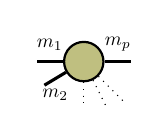
\begin{tikzpicture}[baseline=-0.5ex]
    \tikzset{tensor/.style = {minimum size = 0.5cm,shape = circle,thick,draw=black,inner sep = 0pt}, edge/.style = {thick,line width=.4mm},every loop/.style={}}
    \def\x{6}
    \node[tensor,fill=green!50!red!50!white] (A) at (\x,0) {$\At$};
    \draw[edge] (A) -- (\x-0.6,0) node [midway,above] {\scalebox{0.7}{\dimcolor{$m_1$}}};
    \draw[edge] (A) -- (\x+0.6,0) node [midway,above] {\scalebox{0.7}{\dimcolor{$m_p$}}};;
    \draw[edge] (A) -- (\x-0.5,-0.3) node [midway, below] {\scalebox{0.7}{\dimcolor{$m_2$}}};;
    \draw[dotted] (A) -- (\x,-0.6);
    \draw[dotted] (A) -- (\x,-0.6);
    \draw[dotted] (A) -- (\x+0.5,-0.5);

    \draw[dotted] (A) -- (\x+0.3,-0.6);
    \end{tikzpicture}
\kron
    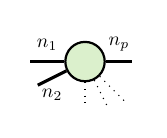
\begin{tikzpicture}[baseline=-0.5ex]
    \tikzset{tensor/.style = {minimum size = 0.5cm,shape = circle,thick,draw=black,inner sep = 0pt}, edge/.style = {thick,line width=.4mm},every loop/.style={}}
    \def\x{6}
    \def\y{0}
    \node[tensor,fill=green!70!red!20!white] (B) at (\x+1,\y) {$\Bt$};
    \draw[edge] (B) -- (\x+0.3,0) node [midway,above] {\scalebox{0.7}{\dimcolor{$n_1$}}};
    \draw[edge] (B) -- (\x+1.6,0) node [midway,above] {\scalebox{0.7}{\dimcolor{$n_p$}}};;
    \draw[edge] (B) -- (\x+0.4,-0.3) node [midway, below] {\scalebox{0.7}{\dimcolor{$n_2$}}};;
    \draw[dotted] (B) -- (\x+1,-0.6);
    \draw[dotted] (B) -- (\x+1.5,-0.5);
    \draw[dotted] (B) -- (\x+1.3,-0.6);
\end{tikzpicture}
=
    \begin{tikzpicture}[baseline=-0.5ex]
    \tikzset{tensor/.style = {minimum width = 3cm,minimum height = 0.6cm,shape = rounded rectangle,thick,draw=black,inner sep = 0pt}, edge/.style = {thick,line width=.4mm},every loop/.style={}}
    \def\x{0}
    \def\y{0}
    \node[tensor,fill=green!30!white] (At) at (\x,\y){$\At\kron\Bt$};
    \draw[edge] (\x-1.25,\y-0.3) -- (\x-1.25,\y-0.6) -- (\x-1.1,\y-0.6) -- (\x-1.1,\y-0.8);
    \draw[edge] (\x-0.85,\y-0.3) -- (\x-0.85,\y-0.6) -- (\x-1,\y-0.6) -- (\x-1,\y-0.8)node [below] {\scalebox{0.7}{\dimcolor{$m_1n_1$}}};
    \draw[edge] (\x-0.65,\y-0.3) -- (\x-0.65,\y-0.6) -- (\x-0.5,\y-0.6) -- (\x-0.5,\y-0.8);
    \draw[edge] (\x-0.25,\y-0.3) -- (\x-0.25,\y-0.6) -- (\x-0.4,\y-0.6) -- (\x-0.4,\y-0.8) node [below] {\scalebox{0.7}{\dimcolor{$m_2n_2$}}};
    \draw[edge] (\x+1.25,\y-0.3) -- (\x+1.25,\y-0.6) -- (\x+1.1,\y-0.6) -- (\x+1.1,\y-0.8);
    \draw[edge] (\x+0.85,\y-0.3) -- (\x+0.85,\y-0.6) -- (\x+1,\y-0.6) -- (\x+1,\y-0.8)  node [below] {\scalebox{0.7}{\dimcolor{$m_pn_p$}}};
    \draw[dotted] (\x+0.1,\y-0.3) -- (\x+0.1,\y-0.6) -- (\x+0.25,\y-0.6) -- (\x+0.25,\y-0.8);
    \draw[dotted] (\x+0.5,\y-0.3) -- (\x+0.5,\y-0.6) -- (\x+0.35,\y-0.6) -- (\x+0.35,\y-0.82) node [below] {\scalebox{0.7}{\dimcolor{$\dots$}}};;
    \end{tikzpicture}
    \in\RR^{m_1n_1\times\dots\times m_pn_p}.
$$

\begin{remark}
下面列出 Kronecker 积的一些有用性质。
\begin{enumerate}
    \item Kronecker 积不满足交换律，即一般地有 $\Ab\kron\Bb \neq \Bb\kron\Ab$%
    . 
    \item
    $
    \Ib\kron\Ab = 
    \begin{bmatrix}
    \Ab & 0 & \dots & 0\\
    0 & \Ab & \dots & 0\\
    \vdots & \vdots & \ddots & \vdots\\
    0 & 0 & \dots & \Ab
    \end{bmatrix}
    $
    是分块对角矩阵。
    \item 两个同阶张量的 Kronecker 积仍是同阶张量，而它们的外积则使阶数翻倍。
    \item 
    对 Kronecker 积 $\Ab\kron\Bb$ 作重排，即可得到外积 $\Ab\outprod\Bb$。
 \item
两个{单位矩阵}的 Kronecker 积是更大的单位矩阵，即 $\Ib_m \kron \Ib_n = \Ib_{mn}$，画出张量网络图便不难看出：
$$
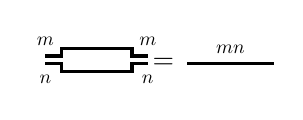
\begin{tikzpicture}[baseline=-0.5ex]
    \tikzset{tensor/.style = {minimum width = 3cm,minimum height = 0.6cm,shape = rounded rectangle,thick,draw=black,inner sep = 0pt}, edge/.style = {thick,line width=.4mm},every loop/.style={}}
    \def\x{0}
    \def\y{0.1}
    \draw[edge](\x-0.1,\y) node [above] {\scalebox{0.7}{\dimcolor{$m$}}}  -- (\x+0.1,\y) -- (\x+0.1,\y+0.1)--(\x+1,\y+0.1) -- (\x+1,\y)-- (\x+1.2,\y) node [above] {\scalebox{0.7}{\dimcolor{$m$}}};
    \draw[edge](\x-0.1,\y-0.1)  node [below] {\scalebox{0.7}{\dimcolor{$n$}}}  -- (\x+0.1,\y-0.1) -- (\x+0.1,\y-0.2)--(\x+1,\y-0.2) -- (\x+1,\y-0.1) --(\x+1.2,\y-0.1)  node [below] {\scalebox{0.7}{\dimcolor{$n$}}} ;
    \node[draw=none] at (\x+1.4,\y-0.1) {\scalebox{1}{\textcolor{black}{$=$}}};
    \draw[edge](\x+1.7,\y-0.1) -- (\x+2.8,\y-0.1) node [midway, above] {\scalebox{0.7}{\dimcolor{$mn$}}} ;
\end{tikzpicture}.
$$
     \item
     两个向量的 Kronecker 积就是它们外积的向量化：
     $$\vectorize(\ub \outprod \vb) = \vectorize(\ub  \vb^\ts) =\ub \kron \vb =  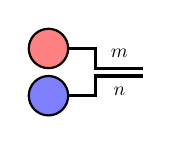
\begin{tikzpicture}[baseline=-0.5ex]
    \tikzset{tensor/.style = {minimum size = 0.5cm,shape = circle,thick,draw=black,inner sep = 0pt}, edge/.style   = {thick,line width=.4mm}}
    \def\x{0}
    \def\y{0}
    \node[tensor,fill=red!50!white] (A) at (\x,\y+0.3){$\ub$};
    \node[tensor,fill=blue!50!white] (B) at (\x,\y-0.3){$\vb$};
    \draw[edge] (\x+0.25,\y+0.3) -- (\x+0.6,\y+0.3) -- (\x+0.6,\y+0.05) -- (\x+1.2,\y+0.05) node [midway,above] {\scalebox{0.7}{\dimcolor{$m$}}};
    \draw[edge] (\x+0.25,\y-0.3) -- (\x+0.6,\y-0.3) -- (\x+0.6,\y-0.05) -- (\x+1.2,\y-0.05) node [midway,below] {\scalebox{0.7}{\dimcolor{$n$}}};
\end{tikzpicture}
    .$$
    \item 
   Kronecker 积满足所谓的\textit{混合乘积}性质：$(\Ab\kron \Bb)(\Cb\kron\Db) = \Ab\Cb\kron\Bb\Db$，其中 $\Ab\in\RR^{m\times n},\Bb\in\RR^{p\times q},\Cb\in\RR^{n\times d}$、$\Db\in\RR^{q\times k}$。
\begin{proof}
 \begin{align*}
(\Ab\kron\Bb)(\Cb\kron\Db) 
&= 
\begin{tikzpicture}[baseline=\baseline]
    \tikzset{tensor/.style = {minimum size = 0.5cm,shape = circle,thick,draw=black,inner sep = 0pt}, edge/.style   = {thick,line width=.4mm}}
    \def\y{0.4}\def\x{0}
    \draw[edge] (\x-1,\y-0.3) -- (\x-0.7,\y-0.3) -- (\x-0.7,\y+0.1)   -- (\x+0.7,\y+0.1) -- (\x+0.7,\y-0.3) -- (\x+1.1,\y-0.3);
    \node[tensor,fill=red!50!white] (A) at (\x,\y){$\Ab$};
    \draw[edge] (\x+1,\y-0.3) -- (\x+1.3,\y-0.3) -- (\x+1.3,\y+0.1)   -- (\x+2.6,\y+0.1) -- (\x+2.6,\y-0.3) -- (\x+3,\y-0.3);
    \node[tensor,fill=orange!50!white] (C) at (\x+2,\y){$\Cb$};
    \def\y{-0.4}\def\x{0}
    \draw[edge] (\x-1,\y+0.4) -- (\x-0.7,\y+0.4) -- (\x-0.7,\y+0.1) -- (\x+0.7,\y+0.1) -- (\x+0.7,\y+0.4) -- (\x+0.7,\y+0.4) -- (\x+1.1,\y+0.4);
    \node[tensor,fill=blue!50!white] (B) at (\x,\y+0.1){$\Bb$};
    \draw[edge] (\x+1,\y+0.4) -- (\x+1.3,\y+0.4) -- (\x+1.3,\y+0.1) -- (\x+2.6,\y+0.1) -- (\x+2.6,\y+0.4) -- (\x+2.6,\y+0.4) -- (\x+3,\y+0.4);
    \node[draw=none] () at (\x+3.25,\y+0.45) {\scalebox{0.7}{\dimcolor{$dk$}}};
    \node[tensor,fill=green!50!red!40!white] (D) at (\x+2,\y+0.1){$\Db$};
    \node[draw=none] () at (\x+1,\y+0.7) {\scalebox{0.7}{\dimcolor{$nq$}}};
    \node[draw=none] () at (\x-1.25,\y+0.4) {\scalebox{0.7}{\dimcolor{$mp$}}};
\end{tikzpicture}\\
 &=
 \begin{tikzpicture}[baseline=\baseline]
    \tikzset{tensor/.style = {minimum size = 0.5cm,shape = circle,thick,draw=black,inner sep = 0pt}, edge/.style   = {thick,line width=.4mm}}
    \def\y{0.4}\def\x{0}
    \draw[edge] (\x-1,\y-0.35) -- (\x-0.7,\y-0.35) -- (\x-0.7,\y)   -- (\x,\y) -- (\x+0.5,\y) -- (\x+0.8,\y);
    \node[tensor,fill=red!50!white] (A) at (\x,\y){$\Ab$};
    \draw[edge] (\x+1.2,\y) -- (\x+1.7,\y) -- (\x+1.7,\y-0.35) -- (\x+2.1,\y-0.35);
    \node[tensor,fill=orange!50!white] (C) at (\x+1,\y){$\Cb$};
    \def\y{-0.4}\def\x{0}
    \draw[edge] (\x-1,\y+0.35) -- (\x-0.7,\y+0.35) -- (\x-0.7,\y) -- (\x,\y) -- (\x+0.8,\y);
    \node[tensor,fill=blue!50!white] (B) at (\x,\y){$\Bb$};
    \draw[edge] (\x+1,\y) -- (\x+1.7,\y) -- (\x+1.7,\y+0.35) -- (\x+2.1,\y+0.35);
    \node[draw=none] () at (\x+2.35,\y+0.4) {\scalebox{0.7}{\dimcolor{$dk$}}};
    \node[tensor,fill=green!50!red!40!white] (D) at (\x+1,\y){$\Db$};
    \node[draw=none] () at (\x-1.25,\y+0.35) {\scalebox{0.7}{\dimcolor{$mp$}}};
    \node[draw=none] () at (\x+0.5,\y+1) {\scalebox{0.7}{\dimcolor{$n$}}};
     \node[draw=none] () at (\x+0.5,\y+0.2) {\scalebox{0.7}{\dimcolor{$q$}}};
\end{tikzpicture}\\
&=
\Ab\Cb\kron\Bb\Db.
    \end{align*}
\end{proof}
特别地，$(\Ab\kron\Ib)(\Ib\kron\Bb)=\Ab\kron\Bb$。 
\item 由上面的推导可以看出，在处理含 Kronecker 积的恒等式时，常常需要把
$
    \begin{tikzpicture}[baseline=\baseline]
    \tikzset{tensor/.style = {minimum size = 0.5cm,shape = circle,thick,draw=black,inner sep = 0pt}, edge/.style   = {thick,line width=.4mm}}
    \def\y{0.6}\def\x{0}
    \draw[edge] (\x+3,\y-0.3)  node [above] {\scalebox{0.7}{\textcolor{gray}{$p$}}} -- (\x+4,\y-0.3)node [above] {\scalebox{0.7}{\textcolor{gray}{$n$}}};
    \def\y{-0.6}\def\x{0}
    \draw[edge] (\x+3,\y+0.3) node [above] {\scalebox{0.7}{\dimcolor{$m$}}}-- (\x+4,\y+0.3)node [above] {\scalebox{0.7}{\dimcolor{$q$}}};
    \end{tikzpicture}
$
重排成
$
 \begin{tikzpicture}[baseline=\baseline]
    \tikzset{tensor/.style = {minimum size = 0.5cm,shape = circle,thick,draw=black,inner sep = 0pt}, edge/.style   = {thick,line width=.4mm}}
    \def\y{0.4}\def\x{0}
    \draw[edge] (\x-1,\y-0.3) -- (\x-0.7,\y-0.3)-- (\x-0.7,\y+0.1) -- (\x+0.7,\y+0.1) -- (\x+0.7,\y-0.3) -- (\x+1.1,\y-0.3);
    \node[draw=none] () at (\x+1.35,\y-0.4) {\scalebox{0.7}{\dimcolor{$nq$}}};
    \node[draw=none] () at (\x-1.25,\y-0.4) {\scalebox{0.7}{\dimcolor{$pm$}}};
    \def\y{-0.4}\def\x{0}
    \draw[edge] (\x-1,\y+0.4) -- (\x-0.7,\y+0.4) -- (\x-0.7,\y+0.1) -- (\x+0.7,\y+0.1) -- (\x+0.7,\y+0.4) -- (\x+0.7,\y+0.4) -- (\x+1.1,\y+0.4);
    \end{tikzpicture}
$，反之亦然。
\item 对 $\Ab\in\RR^{m\times m}$ 与 $\Bb\in\RR^{n\times n},$，有等式 $\tr(\Ab\kron\Bb)=\tr(\Ab)\tr(\Bb)$，由下图不难证明：
$$
\tr(\Ab\kron\Bb) = 
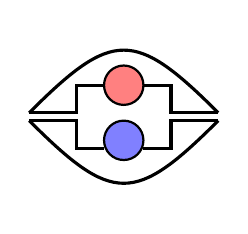
\begin{tikzpicture}[baseline=-0.5ex]
    \tikzset{tensor/.style = {minimum size = 0.5cm,shape = circle,thick,draw=black,inner sep = 0pt}, edge/.style   = {thick,line width=.4mm}}
    \def\x{0}
    \def\y{0}
    \node[tensor,fill=red!50!white] (A) at (\x,\y+0.5){$\Ab$};
    \node[tensor,fill=blue!50!white] (B) at (\x,\y-0.2){$\Bb$};
    \draw[edge] (\x-0.25,\y+0.5) -- (\x-0.6,\y+0.5) -- (\x-0.6,\y+0.15)   -- (\x-1.2,\y+0.15);
    \draw[edge] (\x-0.25,\y-0.3) -- (\x-0.6,\y-0.3) -- (\x-0.6,\y+0.05) -- (\x-1.2,\y+0.05);
    \draw[edge] (\x+0.25,\y+0.5) -- (\x+0.6,\y+0.5) -- (\x+0.6,\y+0.15) -- (\x+1.2,\y+0.15);
    \draw[edge] (\x+0.25,\y-0.3) -- (\x+0.6,\y-0.3) -- (\x+0.6,\y+0.05) -- (\x+1.2,\y+0.05);
    \draw[edge](\x-1.2,\y+0.15) to [out=45,in=135, distance=1.5cm] (\x+1.2,\y+0.15);
    \draw[edge](\x-1.2,\y+0.05) to [out=-45,in=-135, distance=1.5cm] (\x+1.2,\y+0.05);
\end{tikzpicture}
=
\tr(\Ab)\tr(\Bb).
$$

